\section{Theoretical Background}
High harmonic generation (HHG) is an optical phenomenon that involves nonlinear processes wherein laser light frequency is converted into multiple integer multiples. When atoms and molecules are exposed to intense laser fields, typically in the near-infrared range, harmonics of extremely high orders are produced.\cite{hhg-book} We will start by defining some plasma parameters. Then we will give a brief overview of the theory of HHG in gases, followed by a detailed discussion of HHG in plasma.

\subsection{Plasma Parameters}
\subsubsection{Underdense and Overdense Plasma}
Plasma frequency of a plasma with density $n_p$ is given by\cite{chen}
\begin{equation}
    \label{eq:plasma-frequency}
    \omega_p = \sqrt{\frac{n_p e^2}{\epsilon_0 m_e}}
\end{equation}
Let the frequency of the incident laser pulse be $\omega_l$. Now, if $\omega_l > \omega_p$, the plasma is called \textit{underdense}. In this case, the plasma is transparent to the laser pulse. On the other hand, if $\omega_l < \omega_p$, the plasma is called \textit{overdense}. In this case, the laser can not penetrate the plasma and is reflected back. The case $\omega_l = \omega_p$ corresponds to critical plasma and density in this case is called \textit{critical density} $n_c$. Using Equation \ref{eq:plasma-frequency} gives;
\begin{equation}
    \label{eq:critical-density}
    n_c = \frac{\epsilon_0 m_e \omega_l^2}{e^2}
\end{equation}

\subsubsection{Relativistic Laser Pulse}
For a laser of frequency $\omega_l$ and electric field amplitude $E_0$, the laser vector potential is defined as
\begin{equation}
    \label{eq:vector_potential}
    a_0 = \frac{eE_0}{m w_l c}
\end{equation}
A laser is called relativistic if $a_0 \ge 1$. In this situation, the intensity of laser becomes very high and it starts to drive the charged particle it interacts with by relativistic speeds.

\subsection{HHG in Gases}
% HHG in gases occur when an intense laser pulse is focused on gases. When the light photon interacts with atom of gases, three types of ionization occurs depending on the frequency and intensity of the light: if the energy of photon is greater or just equal to the atom ionization potential, then photon ionization occurs. If energy of laser is lss than the atom ionization potential then multiphoton ionization and tunneling ionization occur. Multiphoton and tunneling ionization are two limiting cases of the universal process of nonlinear ionization and this process is determined by three parameters: the laser frequency \(\omega\) , the amplitude of the laser field strength $F$, and the atomic ionization potential \(I_p\).

% \begin{enumerate}
%     \def\labelenumi{\arabic{enumi}.}
%     \item \textbf{In the multiphoton limit} the ionization rate depends on the field strength according to the power law: \[\Omega = F^{2K}\] where K = \textless{}\(I_p\)/\(\Omega\) +1\textgreater{} is the number of absorbed photons
%     \item \textbf{In the tunneling limit} the ionization rate increases exponentially with the field strength \[\Omega \propto  \exp(-2(2I_p)^{3/2}/3F)\]
% \end{enumerate}

% Delone et al.\cite{gas-second} showed that the boundary between multiphoton and tunneling ionization is determined by the value of the adiabaticity parameter:
% \begin{equation}
%     \label{eq:adiabatic}
%     \gamma =\Omega \sqrt{2I_p/F}
% \end{equation}
% \noindent
% $\gamma^2 \gg 1$ correspond to multiphoton ionization, realized at a relatively high frequency and low field strength of laser radiation. On the other hand, the values of $\gamma^2 \ll 1$  correspond to tunneling ionization, which is realized at a low frequency and high field strength.

% HHG in gases occurs when an intense laser pulse interacts with gases. Three types of ionization occur, depending on the frequency and intensity of the light. If the energy of the photon is greater or just equal to the atom ionization potential, then photon ionization occurs. However, if the energy of the laser is less than the atom ionization potential then multiphoton ionization and tunneling ionization occur. Multiphoton and tunneling ionization are determined by the laser frequency \(\omega\), the amplitude of the laser field strength $F$, and the atomic ionization potential \(I_p\). In the multiphoton limit, the ionization rate follows a power law, while in the tunneling limit, the ionization rate increases exponentially with field strength. The adiabaticity parameter, given by

HHG phenomena take place when gases are subjected to the influence of an intense laser pulse. The interaction leads to three different types of ionization, which are dependent on the intensity and frequency of the light. If the photon's energy is equal to or greater than the ionization potential of the atom, photon ionization will occur. On the other hand, if the laser's energy is lower than the ionization potential of the atom, multiphoton ionization and tunneling ionization will occur instead. The determination of multiphoton and tunneling ionization depends on the atomic ionization potential $I_p$, the laser frequency $\omega$, and the amplitude of the laser field strength $F$. In the multiphoton limit, the rate of ionization follows a power law, whereas in the tunneling limit, it increases exponentially as the field strength increases. The adiabaticity parameter, given by
\begin{equation}
    \label{eq:adiabatic}
    \gamma =\Omega \sqrt{2I_p/F}
\end{equation}
determines the boundary between multiphoton and tunneling ionization, with high values corresponding to multiphoton ionization and low values to tunneling ionization. To be precise, $\gamma^2 \gg 1$ corresponds to multiphoton ionization and $\gamma^2 \ll 1$ to tunneling ionization.\cite{gas-second}

\subsubsection{Three Step Model}

In three-step model, we treat the motion of electron initially using quantum mechanics. After it tunnel ionizes from the parent atom, we treat its subsequent dynamics classically. The HHG occurs in three steps:

\begin{figure}[h]
    \centering
    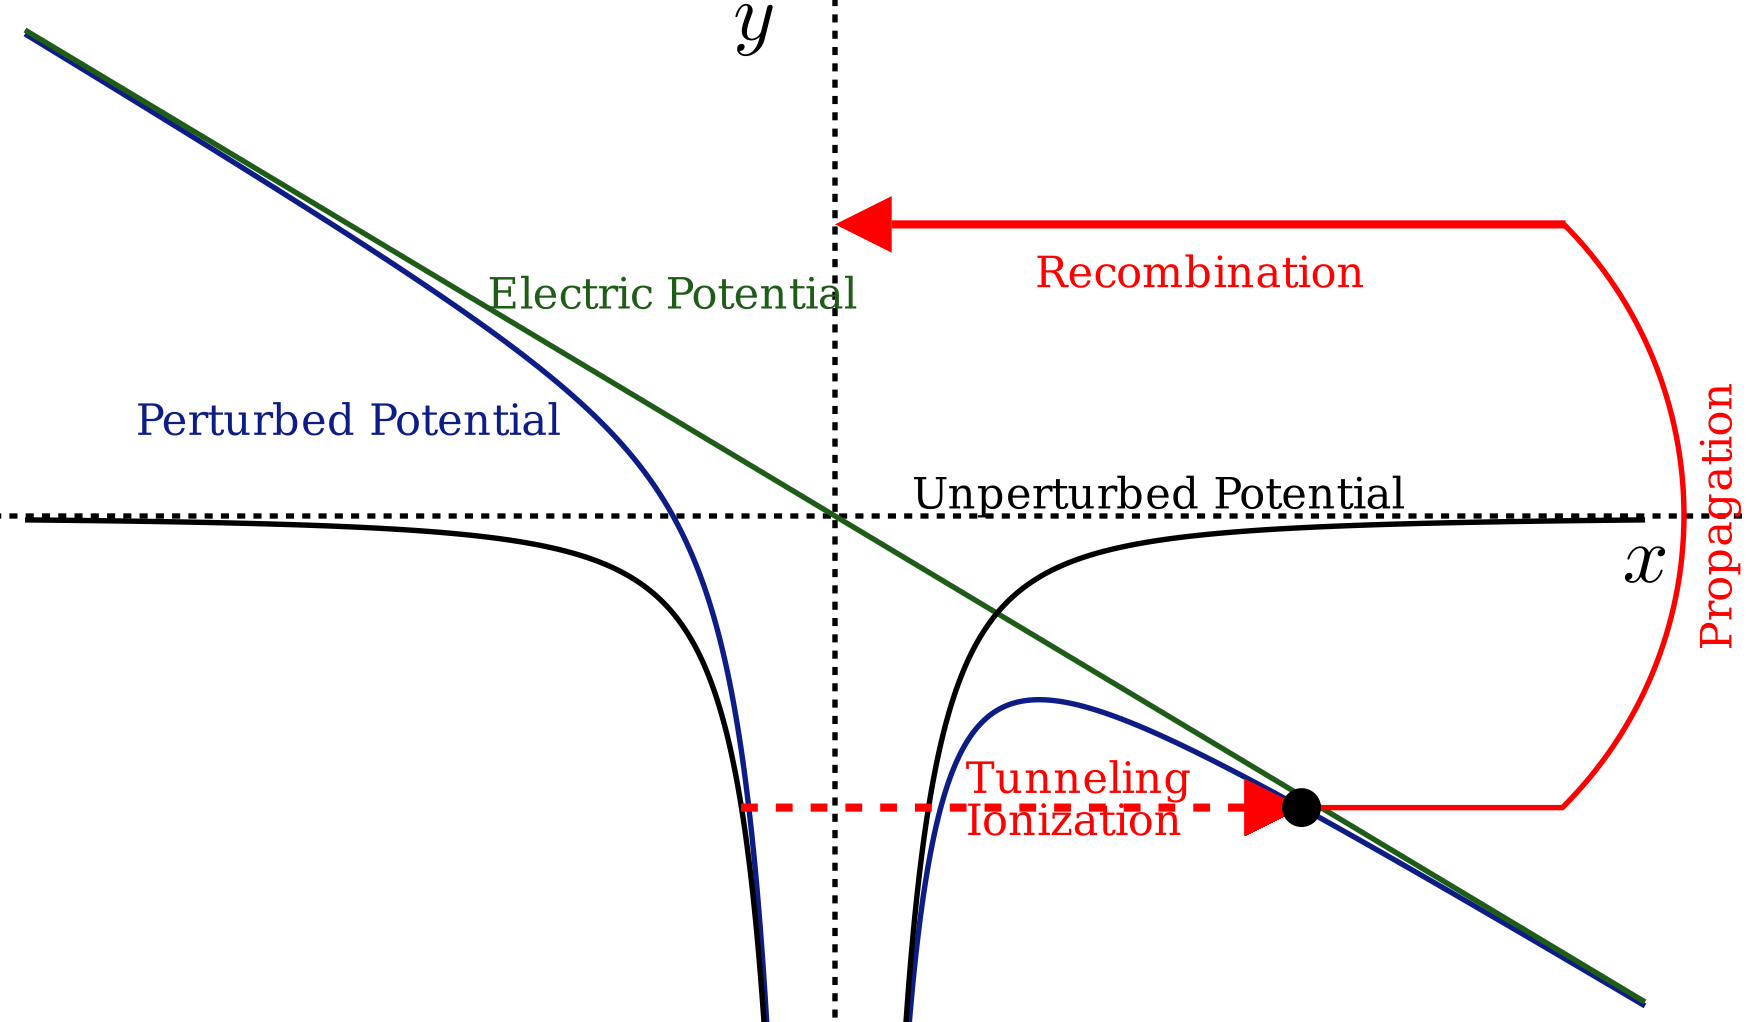
\includegraphics[width=0.7\textwidth]{three_step_one.png}
    \caption{Three steps and fields. The solid black line in the figure shows the binding potential well. The green line is the potential due to the laser field while the solid blue line is the potential created by the instantaneous laser field along with the binding potential well.\\All the illustrations in this sections, if not stated otherwise, are made by the authors using manim\cite{manim}.}
    \label{fig:3-step-1}
\end{figure}
\begin{enumerate}
    \item \textbf{Tunnel ionization} The laser field, which we have assumed to be linearly polarized along the $x$-axis, gives a potential in the form of \(\hat V_L(t)-xFcos(\omega_Lt)\), that is, the potential is proportional to $-x$. This is drawn in figure \ref{fig:3-step-1} as the green line. When this potential couples with the original potential well (in the black line), the potential is deformed (the blue line), called barrier suppression. Electron tunnels through this potential well.
    \item \textbf{Free propagation in the presence of the field} After tunneling, the electron is considered to have no initial velocity as it enters the vacuum. It then experiences acceleration from the electric field of the laser beam. About half a cycle after being ionized, the electron changes direction and moves back toward the parent nucleus due to the reversal of the electric field's direction. During this process, the electron continues to be accelerated.
    \item \textbf{Recollision and recombination} Next, the electron will collide with the nucleus which is the recombination process. During recombination, while the electron returns to its ground state, it can emit radiation of frequency that are multiple of the laser intensity. This is how high harmonics are generated.
\end{enumerate}


\begin{figure}[h]
    \centering
    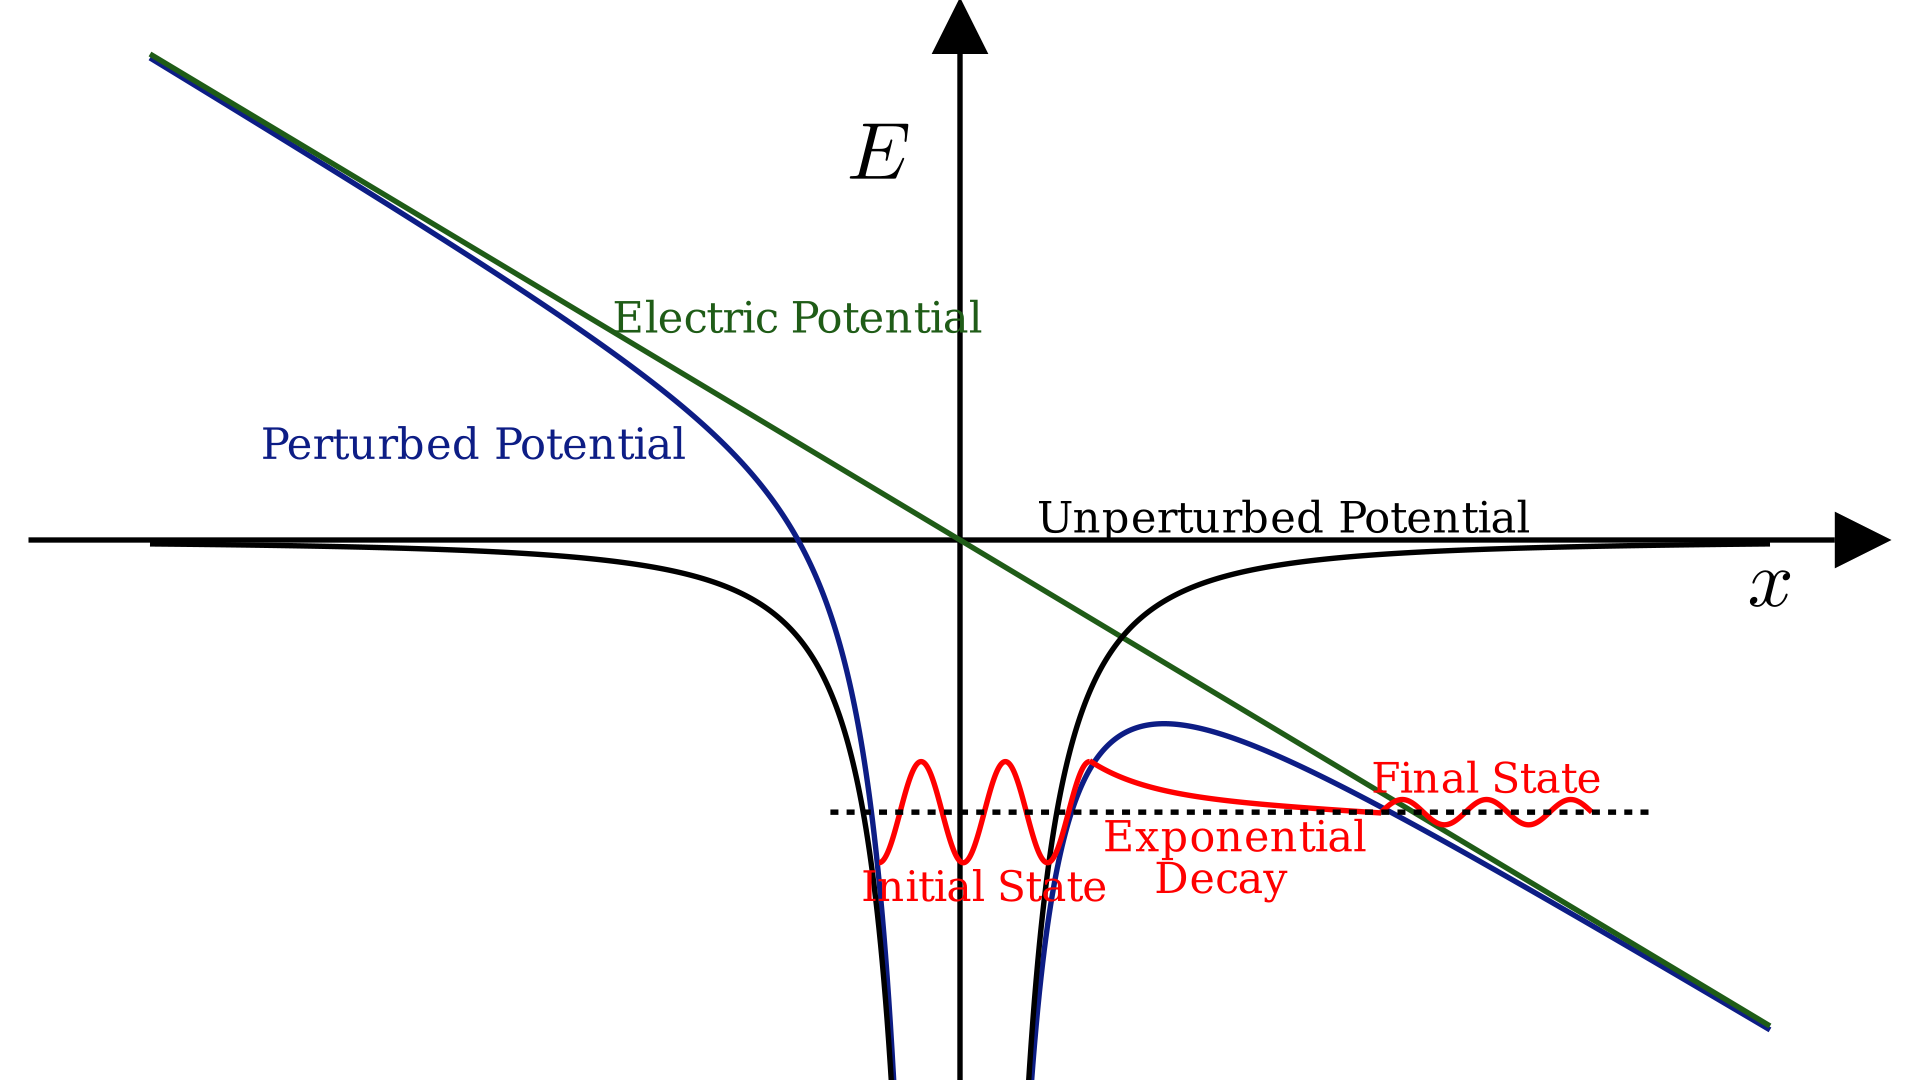
\includegraphics[width=0.7\textwidth]{three_step_two.png}
    \caption{The wave functions of electrons (the red lines). Initially, it is in a potential well. While tunneling, the wave function decay exponentially. After the electron has tunneled through the barrier, it behaves like a free particle with a wave function specified by a smaller amplitude.}
    \label{fig:3-step-2}
\end{figure}

\subsection{HHG in Plasma}
The spectrum from HHG consists of several of integer harmonics of the incident laser pulse (with their intensities decreasing), followed by a plateau, a region, where the harmonic intensity is almost constant over many orders and finally a sharp cutoff. Several of models and theories have been proposed explaining this power law and cutoff. Bezzerides et al.\cite{hhg-relativistic} gave the first model way back in 1983. Their model was based on the relativistic equation of motion and hydrodynamics approximation. They found a cutoff frequency as
\begin{equation}
    \label{eq:cutoff-relativistic}
    n_{\max}^2 = \frac{n_p}{n_c}
\end{equation}
where $n_p$ is the plasma density and $n_c$ is the critical density. The authors showed that the main cause of high-harmonic emission is the powerful nonlinear restoring force that arises during resonant absorption in a density profile that is extremely steep. However, this model was not able to explain the plateau region as well as the fact that we get harmonics that are much higher than the cutoff frequency given by Eq. \ref{eq:cutoff-relativistic}.

\subsubsection{Oscillating Mirror Model}
% To induce large intensity boosts on the reflected laser beam, plasma mirrors need to be set in relativistic motion, which is possible when they are exposed to laser intensities ranging from at least $10^{18} W/cm^2$ up to the highest laser intensities available to date, of a few $10^{22} W/cm^2$. The incident laser field then drives a periodic oscillation of the plasma mirror surface, at relativistic velocities. This relativistic oscillating mirror induces a periodic Doppler effect on the reflected field. Each time the mirror surface moves outward, it compresses the laser energy in time, leading to a sharpening of the reflected waveform. Although still periodic in time, this waveform is no longer sinusoidal: its spectrum thus consists of the combination of the laser frequency $\omega_p$ with a comb of high-order harmonics of frequencies $n\omega_p$.
The concept underlying this model is that the incident laser field induces a periodic oscillation of the plasma mirror surface at relativistic speeds. This oscillating mirror at relativistic speeds results in a periodic Doppler effect on the reflected field, which is responsible for the occurrence of HHG. In this model, it is assumed that the duration of the light pulse is brief enough for the motion of the ions to be disregarded. The ions are considered as a static positive background charge. Additionally, the details of changes in the electron density profile are ignored, and the collective motion of the electrons is represented by the motion of the boundary of the supercritical region. This boundary serves as an effective reflective surface that undergoes oscillatory motion, which is referred to as the oscillating mirror. Using these assumptions, we follow von der Linde et al.\cite{hhg-main} to derive the spectrum of HHG. First, we show that the HHG can be understood as a phase modulation due to the moving mirror.

For this, assuming retardation can be neglected for a moment, the phase shift of the reflected wave caused by a sinusoidal displacement of the reflecting surface in the z-direction is affected.

\begin{equation*}
    s(t) = s_0 \sin(\omega t)
\end{equation*}

is given by
\begin{equation*}
    \phi(t) = (2\omega_0s_0/c)\cos\alpha \sin \omega_m t
\end{equation*}

where $\alpha$ is the angle of incidence and $\omega_m$ is the mirror frequency (modulation frequency). The reflected wave has the elecctric field as:

\begin{equation}
    E_R \propto e^{-i\omega_0 t}e^{i\phi(t)} =  e^{-i\omega_0 t} \sum _{n \to -\infty}^{n \to -\infty}J_n(\chi) e^{-in\omega_m t}
\end{equation}

with $J_n(\xi)$ being the Bessel function of order $n$ and
\begin{equation}
    \label{eq:chi-def}
    \chi = \frac{2\omega_0s_0\cos\alpha}{c}
\end{equation}

% This shows that the phase modulation produced by the oscillating mirror gives rise to a series of sidebands at distances from the carrier frequency $\omega_0$ given by multiples of the modulation frequency $\omega_m$.

% The reflecting surface performs a periodic motion at a frequency $2\omega_0$, or a superposition of $\omega_0$ and $2\omega_0$ , depending on the polarization and angle of incidence of the incoming light. Thus, the modulation frequencies provided by the mirror motion are $\omega_m = \omega_0$ and/or $\omega_m = 2\omega_0$. The key point is that this type of modulation produces sidebands representing even and odd harmonics of the fundamental frequency $\omega_0$ . These ideas suggest an interpretation of high-order harmonic generation from a plasma-vacuum interface as a phase modulation from a periodically moving reflecting surface.

The reflecting surface undergoes periodic motion at a frequency of $2\omega_0$, or a superposition of $\omega_0$ and $2\omega_0$, depending on the polarization and the incidence angle of the incident light. As a result, the modulation frequencies generated by the mirror motion are $\omega_m = \omega_0$ and/or $\omega_m = 2\omega_0$. The crucial point is that this type of modulation gives rise to sidebands representing even and odd harmonics of the fundamental frequency $\omega_0$. These concepts propose an explanation of high-order harmonic generation from a plasma-vacuum interface as a phase modulation from a reflecting surface that moves periodically.

\subsubsubsection{p- and s-Polarization}\label{section:selection}
\begin{figure}[h]
    \centering
    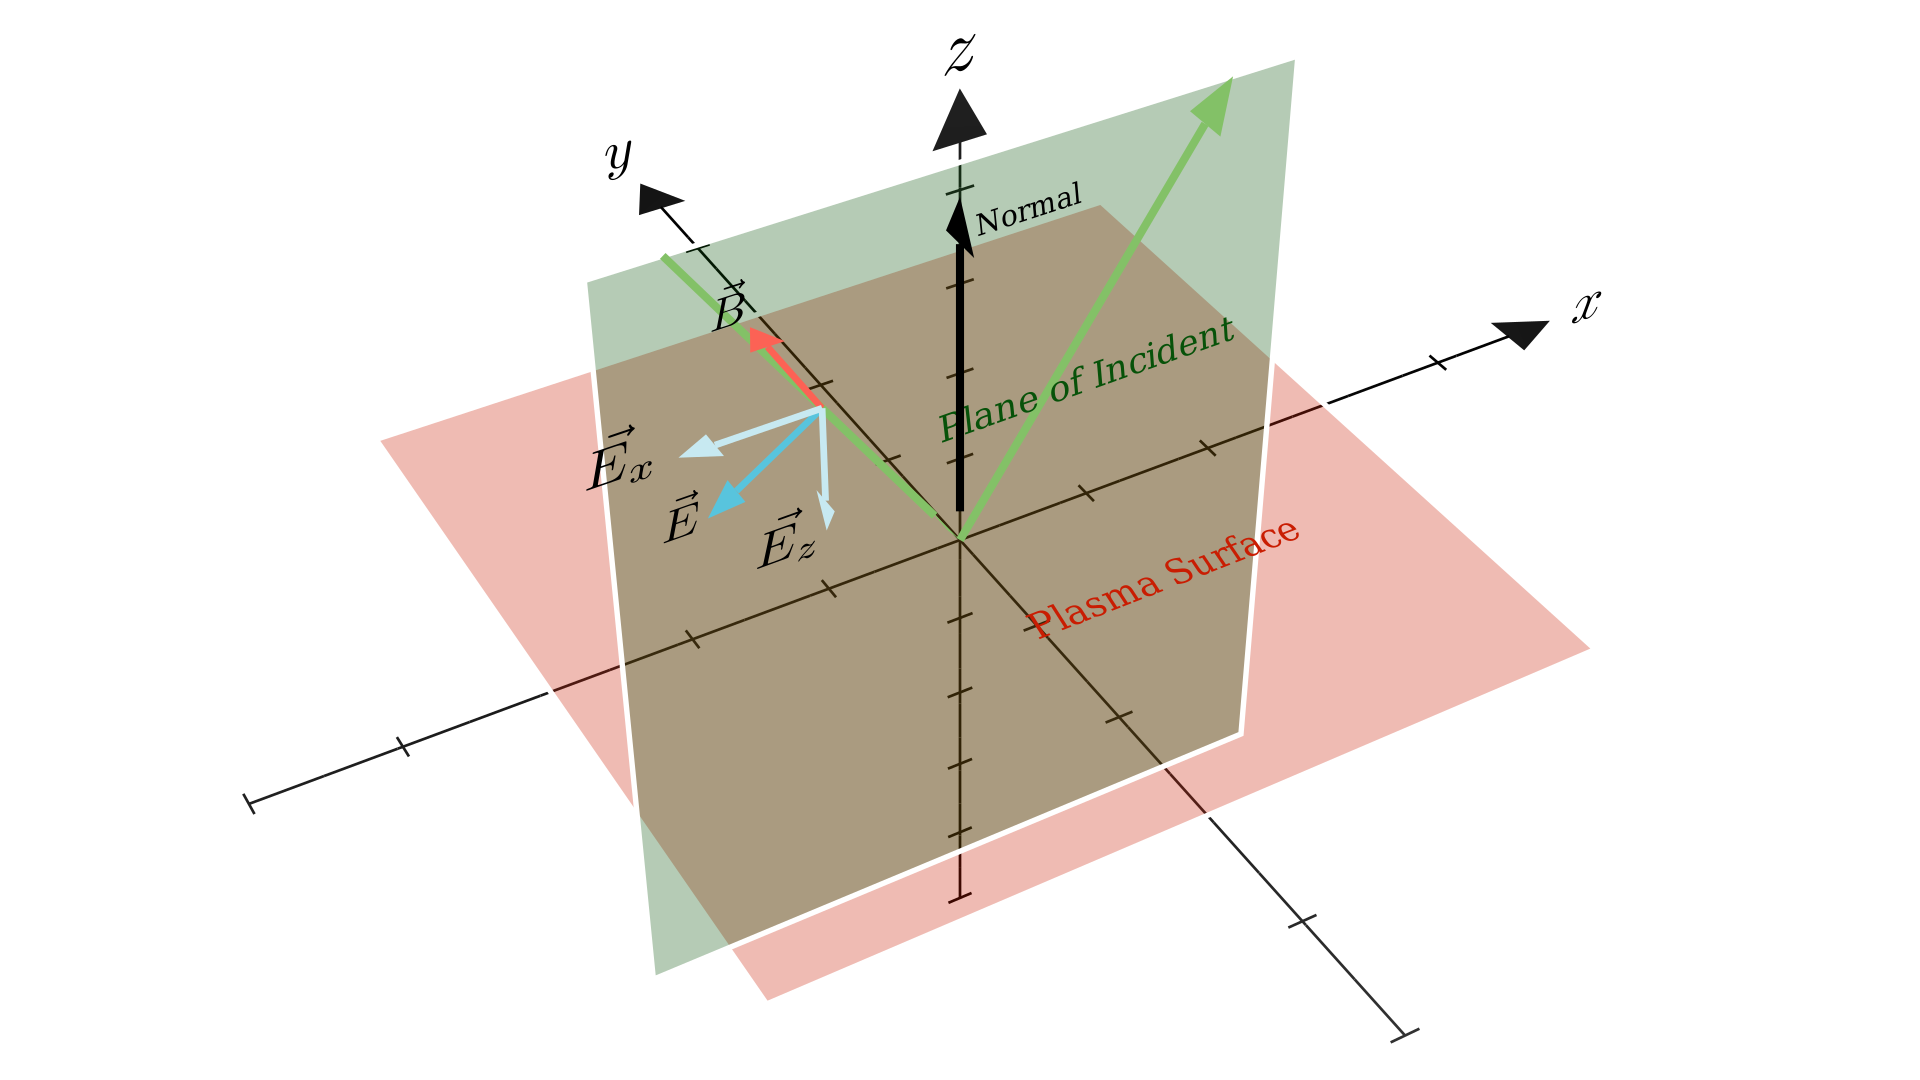
\includegraphics[width=1\textwidth]{p.png}
    \caption{p-polarization. The electric and magnetic fields are parallel and perpendicular, respectively, to the plane of incidence. The motion of the electrons occurs within the plane of incidence.}
    \label{fig:p-polarized}
\end{figure}

\begin{itemize}
    % \item \textbf{p-Polarized Light}: The electric and magnetic fields are, respectively, parallel and perpendicular to the plane of incidence. The electrons move in the plane of incidence. The electron boundary is driven at frequencies $\omega_0$ and $2\omega_0$ , because both the transverse and the longitudinal component of the electron velocity contribute to the motion of the boundary. It follows that in this case both even and odd harmonics with p-polarization are generated. See Fig. \ref{fig:p-polarized}.
    \item \textbf{p-Polarized Light}: In this case, the electric and magnetic fields are parallel and perpendicular, respectively, to the plane of incidence. The motion of the electrons occurs within the plane of incidence. The electron boundary is driven at frequencies $\omega_0$ and $2\omega_0$, as both the transverse and longitudinal components of the electron velocity contribute to the motion of the boundary. As a result, both even and odd harmonics with p-polarization are produced in this scenario. Please refer to the Figure \ref{fig:p-polarized}.
          % \item \textbf{s-Polarized Light}: The electric field is parallel to the plasma-vacuum interface. The electrons move in a plane perpendicular to the plane of incidence. In this configuration only the longitudinal component contributes, while the transverse component of the electron motion is ineffective. The normal motion of the mirror is driven at one frequency only, $\omega_m = 2\omega_0$. It follows that the reflected light is composed of s-polarized odd harmonics and p-polarized even harmonics. See Fig. \ref{fig:s-polarized}.
    \item \textbf{s-Polarized Light}: Here, the electric field of the incident light is parallel to the plasma-vacuum interface, while the electrons move in a plane perpendicular to the plane of incidence. In this setup, only the longitudinal component of the electron motion contributes to the mirror motion, while the transverse component is ineffective. Consequently, the mirror motion is driven at a single frequency, $\omega_m = 2\omega_0$. As a result, the reflected light consists of odd harmonics with s-polarization and even harmonics with p-polarization. Please refer to the Figure \ref{fig:s-polarized}.
          \begin{figure}[h]
              \centering
              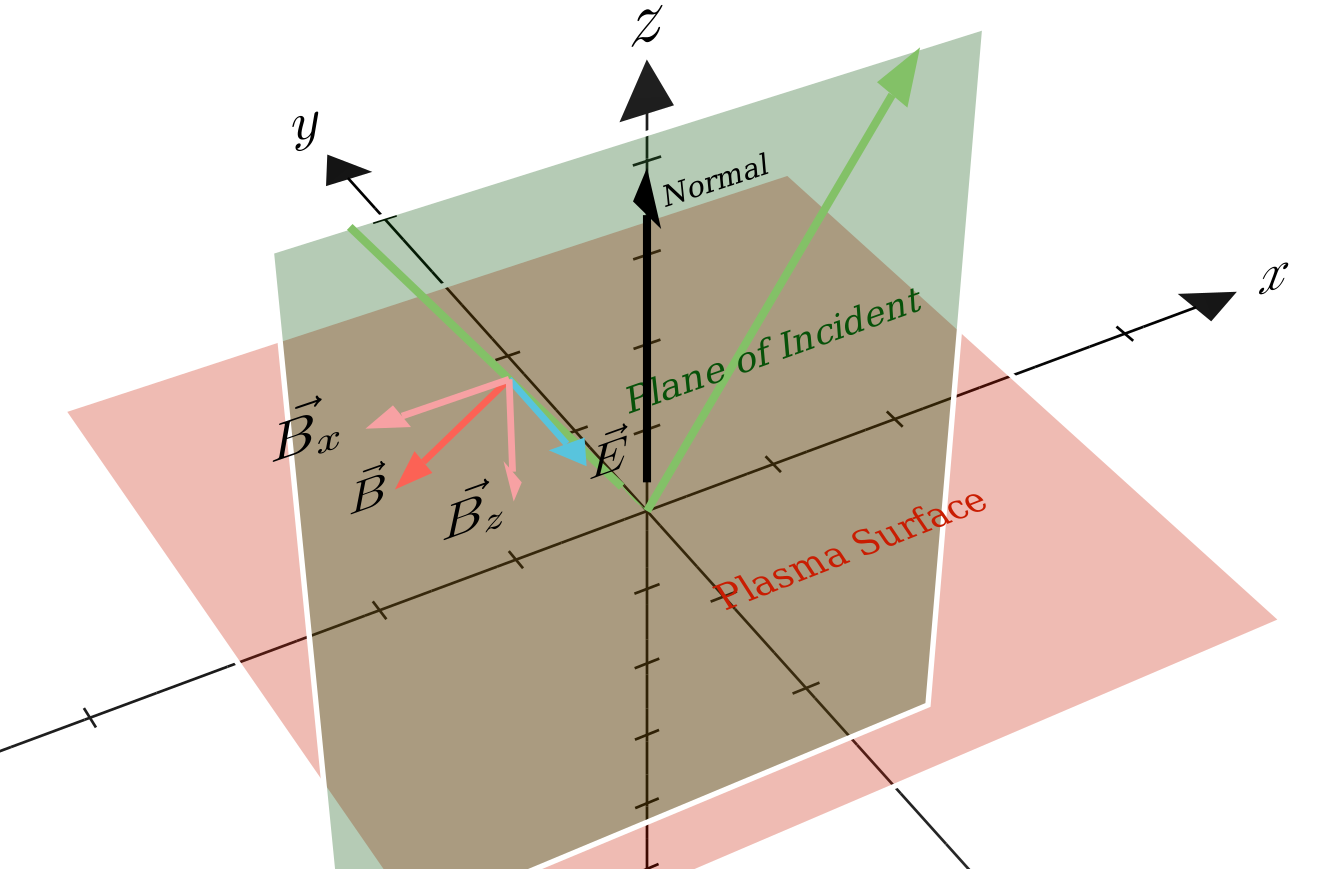
\includegraphics[width=1\textwidth]{s.png}
              \caption{s-polarization. The electric field of the incident light is parallel to the plasma-vacuum interface, while the electrons move in a plane perpendicular to the plane of incidence. }
              \label{fig:s-polarized}
          \end{figure}
\end{itemize}

\begin{table}[h]
    \centering
    \caption{Selection Rule for Polarization}
    \vspace{0.5cm}
    \label{tab:selection-rule}
    \begin{tabular}{|l|l|l|}
        \hline
                                         & \textbf{s-polarized Harmonics} & \textbf{p-polarized Harmonics} \\ \hline
        \textbf{s-Polarized Fundamental} & Odd                            & Even                           \\ \hline
        \textbf{p-Polarized Fundamental} & None                           & Odd and Even                   \\ \hline
    \end{tabular}
\end{table}

\subsubsubsection{HHG Spectrum}
We chose the coordinate system shown in Fig. \ref{fig:s-polarized}. The incident light is polarized along the $y$-axis. The incident light has electric field in the form of:
\begin{equation*}
    E(t, x, z) = E_0 \exp\left(-i\omega_0\left(t-x/c \sin\alpha - z/c \cos\alpha\right)\right)
\end{equation*}

We assume the surface oscillations to be of the form:
\begin{equation*}
    s(t) = s_0 \sin\left( \omega_m \left(t - x/c \sin\alpha\right) \right)
\end{equation*}

The maximum displacement of the surface is $s_0$ is bounded and it is determined by the fact that the velocity must not exceed the speed of light $c$. For example, for s-polarization, as $\omega_m = 2 \omega_0$, we have
\begin{align*}
    s_0 < \frac{c}{\omega_0} & = \frac{c}{2\omega_0} \\
    \therefore \chi          & < \cos\alpha
\end{align*}

% We assume that the reflected wave can be written in the general form of a plane wave propagating in the specular direction:

% \begin{equation*}
%     E_R = G(u) = G(t - x/\sin\alpha + z/\cos\alpha)
% \end{equation*}

% If we further assume that the surface is completely reflecting, then $G(u)$ is obtained from the condition that the total field must vanish on the reflecting surface $z = s(t,x)$, that is:
% \begin{equation}
%     \label{eq:bc}
%     E(t,x,s(t,x)) + E_R(t,x,s(t,x)) = 0
% \end{equation}

In our analysis, we make the assumption that the reflected wave can be expressed as a plane wave propagating in the direction of specular reflection, given by:

\begin{equation*}
    E_R = G(u) = G(t - x/\sin\alpha + z/\cos\alpha)
\end{equation*}

Assuming that the reflecting surface is perfectly reflecting, the function $G(u)$ is determined by the requirement that the total field must be zero at the reflecting surface $z = s(t,x)$. This condition can be expressed as:

\begin{equation}
    \label{eq:bc}
    E(t,x,s(t,x)) + E_R(t,x,s(t,x)) = 0
\end{equation}

We observe that both the sides of the Eq. \ref{eq:bc} are function only of $\xi = t - x/c \sin\alpha$. The spectrum of the reflected wave can be obtained by using the Fourier transform of $G(u)$:
\begin{equation*}
    G(\omega) = \int_{-\infty}^{\infty} G(u) e^{-i\omega u} du
\end{equation*}

where $u = \xi - s_0/c \cos\alpha \sin(\omega_m \xi)$ Integrating, this comes out to be:
\begin{equation}
    \label{eq:G_omega}
    G(\omega) = -2 \pi E_0 \sum_{-\infty}^{+\infty} \frac{1}{1+ n\omega_m /2 \omega_0} \times J_n \left(\left( 1+ n\omega_m /2\omega_0\right)\xi\right)\delta \left(\omega - \omega_0 - n\omega_m\right)
\end{equation}

with $J_n$ being the the Bessel function of order n.

\begin{figure}[h]
    \centering
    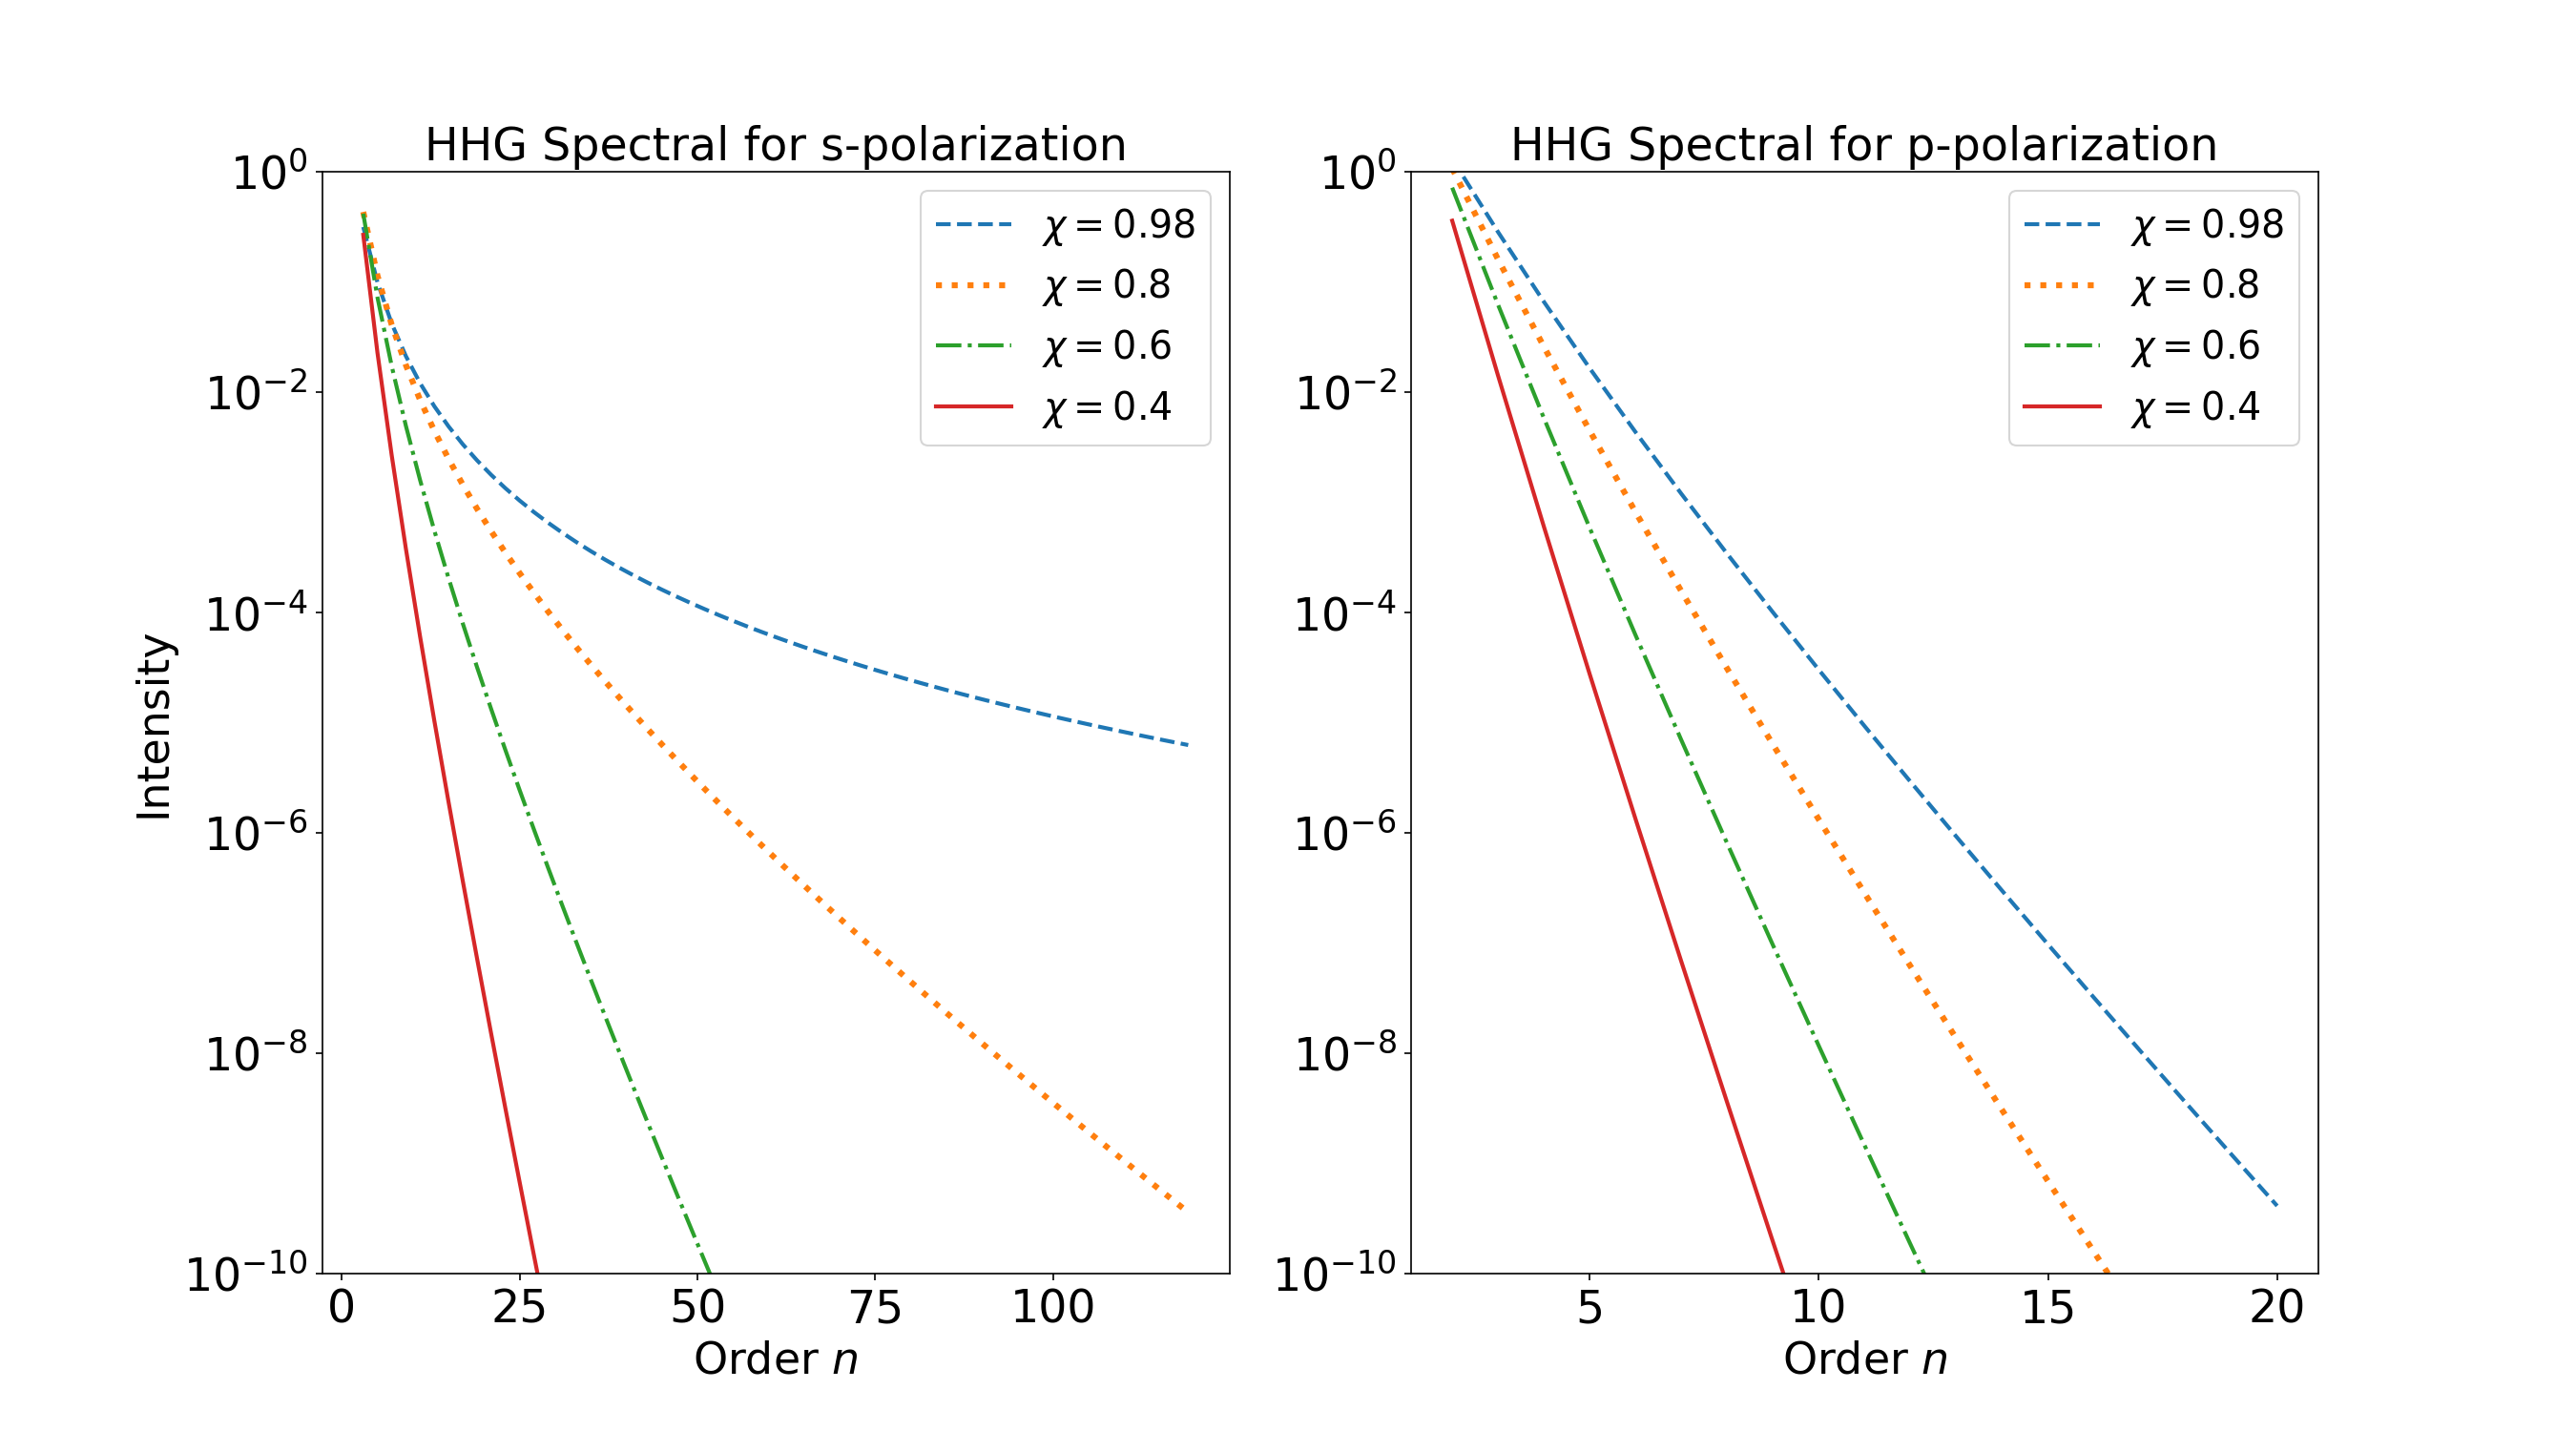
\includegraphics[width=0.85\textwidth, height=7cm]{spectrum.png}
    \caption{HHG spectrum for s and p polarization. The amplitudes of HHG is decreasing more rapidly for p-polarization than s-polarization}
    \label{fig:spectrum}
\end{figure}

For an s-polarization we have, $\omega_m = 2 \omega_0$ and hence equation \ref{eq:G_omega} reduces to:
\begin{equation}
    \label{eq:s-spectrum}
    S((2n+1)\omega_0) = (\pi E_0)^2\left(\frac{J_n((n+1)\xi)}{(n+1)}- \frac{J_{n+1}(n\xi)}{(n)}\right)^2
\end{equation}

For a p-polarization:
\begin{equation}
    \label{eq:p-spectrum}
    S(n\omega_0) = (\pi E_0)^2\left(\frac{J_{n-1}(\frac{1}{2}(n+1)\xi)}{\frac{1}{2}(n+1)}- \frac{J_{n+1}\frac{1}{2}((n-1)\xi)}{\frac{1}{2}(n-1)}\right)^2
\end{equation}

A plot of the spectra is shown in figure \ref{fig:spectrum}.
\subsubsection{Universal Spectra}
The \textit{ideal mirror} assumptions made by von der Linde et al.\cite{hhg-main} are not held in practice. In fact, an ideal mirror is not physically possible. Gordienko et al.\cite{universal-spectra} showed that it is not necessary to assume a form of plasma surface oscillation if the goal is just to get the cutoff and power law of the HHG spectrum. Assuming only the boundary condition equation \ref{eq:bc} and the periodicity of the surface motion, they found the following results which are valid for any type of plasma surface motion:
\begin{enumerate}
    \item The power law for monochromatic wave
          \begin{equation}
              \label{eq:power-law-u}
              I_n \propto 1/n^{5/2}
          \end{equation}
    \item The power law for broadband wave
          \begin{equation*}
              I_n \propto 1/n^{5/2}
          \end{equation*}
    \item The cutoff
          \begin{equation}
              \label{eq:cutoff-u}
              n_c \propto 4\gamma_{\max}^2
          \end{equation}
\end{enumerate}
